\chapter{Dise\~no jer\'arquico de tipos de datos abstractos}

\section{Introducci\'on y noci\'on}

En la etapa de especificaci\'on de problemas, lo \'unico que hemos hecho es detallar qu\'e debemos hacer, pero no nos hemos preocupado por c\'omo hacerlo, es decir que el objetivo era describir el comportamiento del problema a resolver, pero no interesaba determinar c\'omo lo resolver\'iamos. Esto significa que al especificar estamos describiendo el problema, reci\'en al dise\~nar comenzamos a resolverlo.

\subsection{Dise\~no}

Al dise\~nar, centraremos nuestro inter\'es tanto en el \'ambito en el que ser\'a usado el tipo abstracto de datos como en los aspectos que se necesitan optimizar de este tipo, los cuales pueden estar dados por requerimientos expl\'icitos de eficiencia temporal o espacial. Sobre la base de esta informaci\'on, a la que llamaremos \textbf{contexto de uso}, dise\~naremos nuestro tipo aprovechando las ventajas que el contexto nos ofrezca y cuidando de responder a los requisitos que nos plantea. Es importante remarcar que un tipo se define por sus funciones antes que por sus valores. La forma en que los valores se representan es menos importante que las funciones que proveen para manipularlos. Los generadores de los tipos describen la forma abstracta de construir elementos, nunca la forma de construirlos o representarlos f\'isicamente.

En esta etapa, al buscarle representaciones menos abstractas al modelo especificado, es donde realmente comenzaremos a aprovechar el nivel de abstracci\'on. Cuanto m\'as abstracto sea el modelo, mas opciones de dise\~no tendremos disponibles en cada paso. B\'asicamente nuestra metodolog\'ia de dise\~no partir\'a entonces de un modelo abstracto no implementable directamente en un lenguaje imperativo de programaci\'on, y aplicar\'a iterativamente sobre dicho modelo sucesivos pasos de refinamiento hasta llegar a estructuras que si son implementables. En cada una de estas sucesivas iteraciones estaremos realizando, de cierta forma, una desabstracci\'on.

~

Es importante tener en cuenta que en la especificaci\'on estaremos centrados en un paradigma funcional y en la etapa de dise\~no nos centraremos en paradigma imperativo, por lo que tendremos un cambio de paradigma adem\'as de la desabstracci\'on del modelo, lo que nos conllevara ciertas dificultades. Uno de los objetivos del lenguaje de dise\~no es justamente permitir un cambio de paradigma que resulte ordenado.

\subsection{Jer\'arquico}

Cada iteraci\'on de desabstracci\'on de este proceso definir\'a un nivel de nuestro dise\~no. Por su parte, cada uno de estos niveles tendr\'a asociado uno o m\'as m\'odulos de abstracci\'on, que indicaran c\'omo se resuelven las operaciones de un m\'odulo utilizando otras operaciones de m\'odulos del nivel inmediato inferior. Cada uno de estos m\'odulos de abstracci\'on resultantes de cada iteraci\'on, ser\'a implementable en un lenguaje de programaci\'on, obteniendo de tal forma un dise\~no estratificado en niveles donde los m\'odulos de un cierto nivel son usuarios de los servicios que les brindan los del nivel inmediato inferior y no conocen (ni usan) a los m\'odulos de otros niveles. Un m\'odulo dar\'a a conocer los servicios que provee a trav\'es de una declaraci\'on de las operaciones que exporte junto con la aridad de cada una de ellas, se dar\'an a conocer las precondiciones (estado esperado de la m\'aquina antes de ejecutarse la operaci\'on) y las postcondiciones (como incidir\'a la ejecuci\'on en 
el estado anterior). Esta informaci\'on estar\'a incluida en la interfaz del m\'odulo.

~

Esta separaci\'on o encapsulamiento en niveles provocara que cualquier cambio de implementaci\'on de nivel $n$ ser\'a transparente al nivel superior $n+1$, siempre que el nivel $n$ mantenga su interfaz. Esto es, que el m\'odulo exporte al menos las mismas funciones que se exportaban antes y la funcionalidad provista por las mismas no cambi\'e, aunque puede haber mejorado su performance. Podremos verificar la validez del cambio de dise\~no viendo que la veracidad de las precondiciones y postcondiciones del nivel redise\~nado se mantiene con respecto a la versi\'on anterior.

\section{Lenguaje de dise\~no}

Este es el lenguaje que utilizaremos para dise\~nar nuestros m\'odulos. El mismo, si bien sera un pseudoc\'odigo, estar\'a muy basado en lenguajes que se utilizan en la vida real, de esta forma la transici\'on desde el dise\~no a los mismos ser\'a casi inmediata.

\subsection{Paradigma imperativo}

Para especificar formalmente el problema a resolver escrib\'iamos el tipo abstracto de datos siguiendo un paradigma funcional. Sin embargo al dise\~nar, debemos realizar un cambio de paradigma para poder expresar nuestra representaci\'on del modelo en un lenguaje imperativo, el cual se ajusta a los lenguajes de programaci\'on mas bastamente usados. En esta secci\'on discutiremos los principales aspectos que deberemos tener en cuenta al afrontar tal cambio.

\subsubsection*{Valores vs. Objetos}

Las aridades de las operaciones que definimos en la especificaci\'on para los tipos est\'an en una notaci\'on funcional, esto quiere decir que supone que las mismas construyen un objeto nuevo y lo devuelven a aquel que las llamo. Una caracter\'istica de esta notaci\'on es la transparencia referencial, esto es que una expresi\'on siempre da el mismo resultado sin importar su contexto. En este paradigma los datos s\'olo tienen sentido en cuanto sean argumentos o resultados de funciones.

Al contrario del paradigma funcional los datos en el paradigma imperativo son tratados como entidades independientes de las funciones que los utilizan. Es usual que se trabaje con una instancia de un objeto que se va modificando y cuyos valores anteriores no interesen. Por lo tanto, por cuestiones de optimizaci\'on y uso, no tiene sentido construir cada vez un objeto nuevo para devolverlo como resultado de una funci\'on, sino que en cambio se modificara el objeto original.

\subsubsection*{Par\'ametros que se modifican}

El mapeo de los par\'ametros de las funciones del tipo en las operaciones del m\'odulo no siempre es uno. De hecho en el paradigma imperativo se acostumbra a modificar los par\'ametros como parte de respuesta del algoritmo y a devolver en el valor de retorno de la funci\'on, alg\'un estado que informe si la operaci\'on se completo de forma correcta o si hubo alg\'un problema. Esto nos brinda una mayor versatilidad a la hora de dise\~nar las interfaces, ya que una misma funci\'on puede devolver varios tipos de resultados sin necesidad de hacerlo mediante una tupla y adem\'as dar alguna informaci\'on acerca de la ejecuci\'on.

\subsection{Tipos disponibles}

Los tipos listados a continuaci\'on ser\'an considerados tipos b\'asicos y no ser\'an dise\~nados: bool, nat, int, real, char, string, g\'enero, puntero$\langle tipo\_dato \rangle$, arreglo[$nat$] de $tipo\_dato$, tupla$\langle campo_1\:tipo\_dato \times ... \times campo_n\:tipo\_dato \rangle$, arreglo\_dimensionable de $tipo\_dato$.

\subsection{Declaraci\'on de operaciones y pasaje de par\'ametros}

Para declarar las operaciones se le asignara un nombre, se describir\'an los argumentos y los tipos de cada uno como as\'i tambi\'en el tipo de dato del valor de retorno de la funci\'on. El pasaje de par\'ametros puede pertenecer a 3 tipos:

\begin{itemize}
 \item \textbf{entrada} El valor es usado como dato pero no es posible modificarlo (en C++ la equivalencia seria el const). Se denota anteponiendo al nombre de la variable en el tipo de la operaci\'on el s\'imbolo ``\textbf{in}''.
 \item \textbf{salida} El valor se genera en la operaci\'on, y se almacena en el par\'ametro formal con el que se invoc\'o a la funci\'on pero no es usado como dato. Se lo denota con ``\textbf{out}''. La variable resultado (la que devuelve la funci\'on) pertenece a esta categor\'ia.
 \item \textbf{entrada-salida} Combina los conceptos anteriores, se lo denota con ``\textbf{in}/\textbf{out}''.
\end{itemize}

Recordemos que en el paradigma imperativo todos los valores son pasados por referencia, exceptuando a los tipos primitivos (bool, nat, int, real, char, puntero) que son pasados por valor o copia$^*$. Al ser pasados por referencia y al ser del tipo de entrada-salida o salida y efectuar una asignaci\'on sobre el mismo, el valor con el que fue llamada la funci\'on es sobreescrito y el nuevo valor ser\'a el que mantendr\'a la variable luego de salir de la funci\'on, esto quiere decir que la variable que pasamos como par\'ametro de la funci\'on es efectivamente modificada por mas que nos encontremos dentro del scope de la funci\'on.

\textbf{*} En el caso de los arreglos dimensionables y est\'aticos, se pasan por referencia, y en el caso de las tuplas, cada una de sus componentes se pasa por referencia o por copia seg\'un sea un tipo primitivo o no.

\subsection{Asignaci\'on y alising}

La expresi\'on $A \gets B$ (siendo $A$ y $B$ variables de un mismo tipo), denota la asignaci\'on del valor $B$ a la variable $A$. Esto funciona del mismo modo que el pasaje de par\'ametros. Si $A$ y $B$ pertenecen a un tipo primitivo $A$ pasara a ser copia de $B$, y si no son tipos primitivos, luego de haber efectuado la asignaci\'on, $A$ y $B$ har\'an referencia a la misma estructura f\'isica, es decir $A$ sera un alias de $B$ y viceversa (de ah\'i el nombre).

\subsection{Relaci\'on entre el dise\~no y la especificaci\'on, precondiciones y postcondiciones}

Al describir la interfaz de un m\'odulo para cada una de las operaciones deberemos indicar cu\'ales son sus restricciones y qu\'e efectos produce en el estado de la m\'aquina. Para describir esto haremos uso de la especificaci\'on del tipo abstracto de datos asociado al m\'odulo, lo que en consecuencia nos obligar\'a a describir la relaci\'on que existe entre las variables del dise\~no y el tipo abstracto de datos especificado. Queremos poder describir en la interfaz cual es el resultado final luego de aplicada una operaci\'on teniendo en cuenta los par\'ametros con los cuales se la invoca y las relaciones entre ellos.

~

Cuando nos pasa esto tenemos el problema de que los tipos y operaciones a las que queremos hacer referencia est\'an en el mundo de los TADs y por otro lado, las funciones sobre las que queremos describir su entrada y resultado est\'an en el mundo del dise\~no. Por lo que de cierta forma queremos comparar elementos que no est\'an definidos en base a axiomas, con elementos que si lo est\'an. Para subsanar esta dificultad, existir\'a la funci\'on $\widehat{\text{\textbullet}}$.

~

Llamaremos $G_I$ al conjunto de g\'eneros del paradigma imperativo y $G_F$ al conjunto de g\'eneros del paradigma funcional. Sub-indexaremos con $I$ a los g\'eneros de $G_I$ y con $F$ a los de $G_F$. Es decir, disponemos de una funci\'on que dado un g\'enero del paradigma imperativo nos da su ``equivalente'' en el paradigma funcional, la misma quedara definida como:

\begin{equation*}
 \widehat{\text{\textbullet}}: G_I \rightarrow G_F
\end{equation*}

Mediante el uso de esta funci\'on podremos establecer de forma clara el mapeo entre las operaciones del m\'odulo y las funciones de la especificaci\'on cuando escribamos las precondiciones y postcondiciones de cada operaci\'on del m\'odulo.

\newpage

\section{Metodolog\'ia de dise\~no}

Nuestro objetivo es obtener un dise\~no jer\'arquico y modular, para realizar esto hay varias formas pero presentaremos un m\'etodo que tiene las nociones de los distintos niveles en la jerarqu\'ia. Cada uno de los niveles tendr\'a asociado un m\'odulo de abstracci\'on. Para ser m\'as precisos, habr\'a distintos tipos abstractos de datos que deberemos dise\~nar, a cada uno de ellos le corresponder\'a un m\'odulo de abstracci\'on. A grandes rasgos, el m\'etodo se compone de los siguientes pasos:

\begin{itemize}
 \item Elecci\'on del tipo abstracto de datos a dise\~nar.
 \item Implementaci\'on del m\'odulo de abstracci\'on para el tipo abstracto de datos elegido.
 \item Iteraci\'on o finalizaci\'on.
\end{itemize}

\subsection{Elecci\'on del tipo a dise\~nar}

El orden en el cual se dise\~nan los tipos es arbitrario. Sin embargo es una buena pr\'actica comenzar por los tipos m\'as importantes, pues \'estos ser\'an los principales generadores de requerimientos de eficiencia para los tipos menos importantes o de niveles inferiores. De cierta forma estamos aplicando el esquema top-down. Es importante notar que el proceso de dise\~no posee una natural idea y vuelta. Por ejemplo, la redefinici\'on de las funciones de un tipo puede obligarnos a reveer la secci\'on representaci\'on de un tipo que basa su dise\~no en \'este. Si lo vemos desde el punto de vista expl\'icitamente jer\'arquico, la redefinici\'on de las operaciones de un tipo de un nivel, puede obligarnos a redefinir a un modulo de un nivel superior.

~

Cuando dise\~namos un m\'odulo, no necesariamente debemos dise\~nar todos los tipos que usamos en la especificaci\'on. Esto quiere decir que a veces sucede que en la especificaci\'on realizamos ciertas tareas utilizando tipos que en la etapa de dise\~no, al no ser el objetivo la descripci\'on del problema y serlo la resoluci\'on del mismo, podemos no necesitar. Es decir que si tenemos un tipo que no se exporta directamente y solamente necesitamos algunas de sus operaciones, podemos quiz\'as evitar usarlo y reemplazarlo por algo mas ligero que cumpla nuestros requerimientos. Esto expresa que la manera en que se axiomatizan los tipos en el TAD no es importante a la hora de realizar el dise\~no, sino que solamente es importante lo que dichos axiomas significan.

\subsection{Implementaci\'on del m\'odulo de abstracci\'on para el tipo elegido}

Una vez elegido el tipo a dise\~nar, implantaremos su m\'odulo de abstracci\'on correspondiente. El m\'odulo de abstracci\'on deber\'a describir de forma clara y concisa las operaciones que podr\'a realizar, como as\'i tambi\'en los efectos de las mismas sobre los datos, las complejidades temporales y espaciales que tomar\'an su uso y cuales de las operaciones podr\'an ser utilizadas externamente, es decir, cuales se exportar\'an. Adem\'as de dar una descripci\'on externa del mismo poseer\'a otra secci\'on en la cual se explicitar\'a la implementaci\'on de cada una de las operaciones (incluyendo operaciones privadas auxiliares) como as\'i tambi\'en la estructura de datos interna utilizada para llevar al cabo las tareas.

\subsection{Iteraci\'on o finalizaci\'on.}
En este punto tenemos un dise\~no que puede contener tipos para los que no tenemos una propuesta de dise\~no. En realidad son otros problemas a resolver de nivel de abstracci\'on menor al original. Por lo tanto, debemos volver a repetir el m\'etodo con los nuevos tipos a dise\~nar.

La iteraci\'on prosigue hasta llegar a tipos que tengamos dise\~nados en nuestra biblioteca o sean primitivos. Por otro lado, la reutilizaci\'on de tipos ahorra tiempo de dise\~no pero ya que es posible reutilizar tipos que fueron dise\~nados con criterios distintos a los que deseamos, podr\'iamos perder parte de la eficiencia buscada lo que ser\'a tolerable siempre y cuando no rompa las restricciones planteadas por el contexto de uso.

\newpage

\section{M\'odulo de abstracci\'on}

Cada m\'odulo de abstracci\'on est\'a compuesto por dos secciones: la \textbf{definici\'on de la interfaz} y la \textbf{definici\'on de la representaci\'on}. En la \textbf{interfaz} se describe la funcionalidad del m\'odulo y en qu\'e contexto puede ser usado. En la \textbf{representaci\'on} se elige, bajo alg\'un criterio, una forma de representaci\'on utilizando otros m\'odulos y se resuelven las operaciones del m\'odulo en funci\'on de su representaci\'on. Dicho de otra forma, se eligen las estructuras de datos internas que representar\'an el modulo y se implementan los algoritmos que la interfaz expresa. Un m\'odulo de dise\~no debe tener la siguiente estructura:

\begin{SCfigure}[1][ht!]
 \centering
 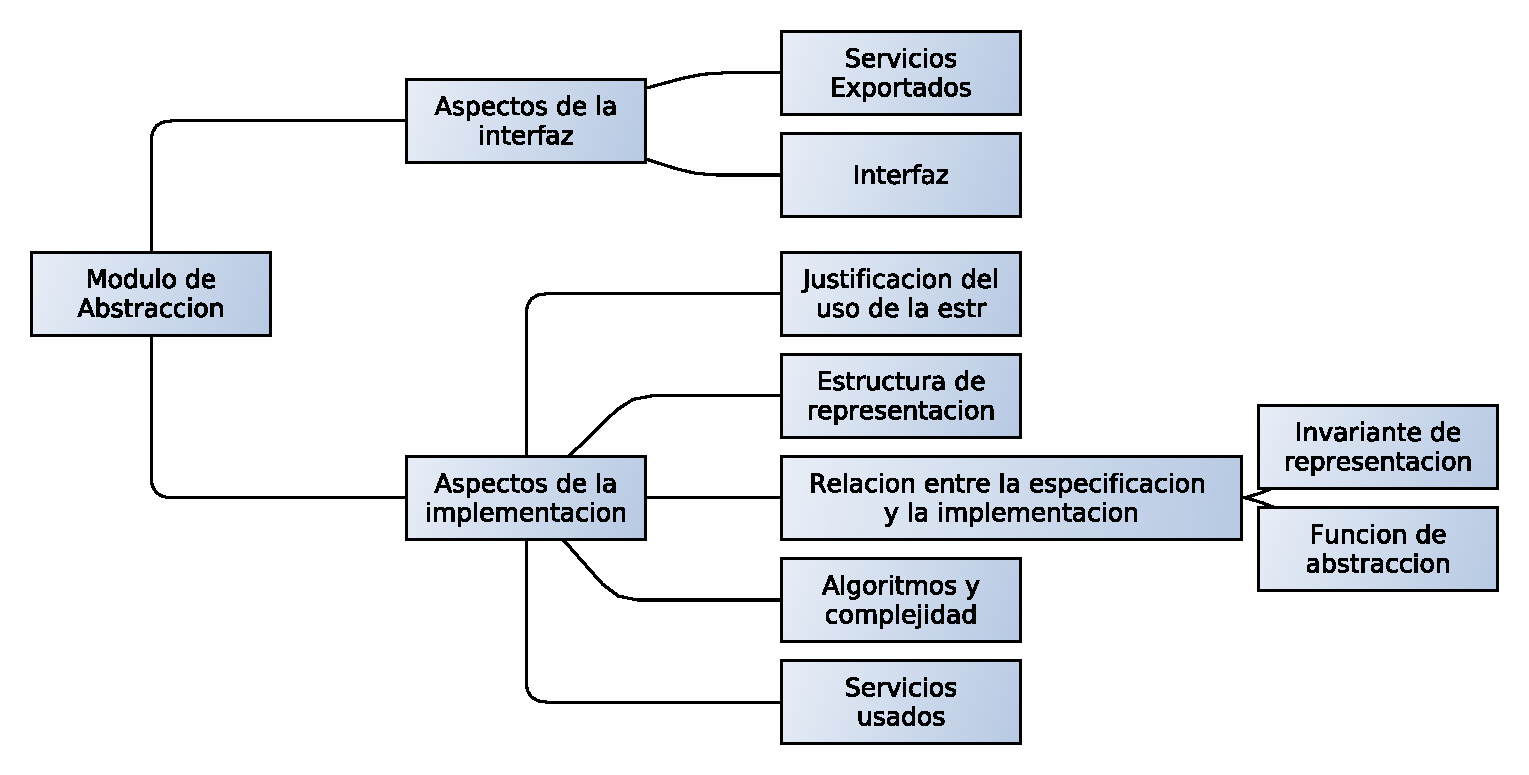
\includegraphics[width=0.7\textwidth]{graficos/ModuloDeDisenio.pdf}
\end{SCfigure}

\begin{itemize}
 \item \textbf{Especificaci\'on} Puede omitirse si es uno de los TADs provistos por la c\'atedra, o incluirse s\'olo los cambios si es una extensi\'on de un TAD ya conocido.
 \item \textbf{Interfaz} La cual contendr\'a los servicios exportados, \'ordenes de complejidad, aspectos de alising, efectos secundarios, etc. En definitiva, todo lo que el usuario necesite saber.
 \item \textbf{Representaci\'on} Estructura interna, invariante, funci\'on de abstracci\'on y algoritmos.
 \item \textbf{Servicios usados} \'Ordenes de complejidad, aspectos de alising, etc. requeridos de los tipos de soporte que utilizamos en nuestro m\'odulo.
\end{itemize}


\subsection{Aspectos de la Interfaz}

En este paso tomamos las decisiones concernientes al cambio de paradigma. Una forma de lograr esto es redefinir las aridades de las funciones adapt\'andolas a un lenguaje imperativo explicitando los requerimientos (precondiciones) para la aplicaci\'on de cada operaci\'on y los efectos que tiene sobre el estado de la m\'aquina (postcondiciones). Para escribir las precondiciones y las postcondiciones usaremos un lenguaje de descripci\'on de estados aprovechando la especificaci\'on del tipo a dise\~nar.

~

Durante la redefinici\'on de aridades no debemos limitarnos a cambiar una operaci\'on por un procedimiento como as\'i tambi\'en a respetar exactamente la cantidad de par\'ametros que tiene una operaci\'on. Siempre podremos decidir usar m\'as de un procedimiento para reemplazar a una operaci\'on del tipo abstracto como as\'i tambi\'en, y contrariamente, tendremos la posibilidad de unir varias funciones del tipo abstracto en una sola del dise\~no. Adem\'as de poder evitar totalmente el mapeo uno a uno podremos incluir funciones que no tengan sentido desde el punto de vista abstracto pero sean \'utiles dentro del paradigma imperativo, por ejemplo funciones para copiar instancias del tipo o funciones como ``comprimir'' cuyos efectos sean visibles solo desde la eficiencia temporal y espacial de las operaciones, pero no signifiquen un cambio en el valor representado. Todas estas decisiones dependen del contexto de uso.

\subsubsection{Servicios exportados / Operaciones exportadas}

En esta secci\'on deben estar expresados los detalles acerca de nuestro m\'odulo que resulten indispensables a sus usuarios. Es imprescindible tocar temas como la complejidad temporal de los algoritmos y cuestiones de alising y efectos secundarios de las operaciones. Adem\'as, pueden exhibirse comentarios (a modo informativo) con respecto a la implementaci\'on del m\'odulo que, aunque tengan menor importancia, sean de inter\'es para el usuario. Los puntos a recalcar que debe tocar esta \'area son los siguientes:

\begin{itemize}
 \item Deducir y documentar la \textbf{complejidad temporal} de cada operaci\'on es fundamental dentro de esta area, ya que de no haber informaci\'on de la misma nuestro m\'odulo no podr\'ia ser utilizado por ning\'un otro m\'odulo cuyo contexto de uso restringiera tal aspecto. Dicho de otra forma, un usuario que deba responder a requerimientos de eficiencia temporal y deba usar nuestro m\'odulo, no podr\'a saber si esta cumpliendo con ellos si no documentamos los mismos.
 \item Conocimiento del \textbf{alising} es de vital importancia para el uso correcto y eficiente del m\'odulo. Si no inform\'asemos las cuestiones de alising referentes a las operaciones podr\'ia pasar que un usuario de nuestro m\'odulo modifique datos sin saberlo por estar utilizando alg\'un alias (en vez de una copia) generado a partir del uso de de una de nuestras operaciones, lo que provocar\'ia un problema muy grave en el desarrollo del programa.
 \item Es importante indicar en las operaciones que \textbf{eliminan elementos de la estructura} si dichos elementos seguir\'an existiendo o ser\'an eliminados. Esto afecta a los usuarios que tengan referencias a dichos elementos. Si se los elimina, las referencias a ellos dejar\'an de ser v\'alidas, en caso contrario seguir\'an vigentes pero ya no estar\'an en la estructura, por lo que ser\'a el usuario el encargado de liberarlas al momento de implementar su m\'odulo ya que de no hacerlo podr\'a producir una potencial perdida de memoria.
\end{itemize}

\subsubsection{Contexto de uso y requerimientos de eficiencia de los servicios prestados}

Como dijimos al inicio, el contexto de uso esta dado por el entorno en donde vaya a ser usado el programa del cual se derivar\'an, a trav\'es de un an\'alisis de las funciones que ser\'an m\'as usadas, los requerimientos de eficiencia y adem\'as que estructuras de datos que se ajustan mejor al contexto en el que se encuentra el dise\~no. No se puede conocer si un dise\~no es adecuado si no se aclara precisamente el contexto de uso. La idea es que la principal justificaci\'on para el resultado obtenido en cada iteraci\'on de dise\~no es el contexto de uso que se le impuso al dise\~nador.

\subsection{Aspectos de la Implementaci\'on}

El objetivo de esta secci\'on es definir la forma en que representaremos el tipo que estamos dise\~nando en esta iteraci\'on (o nivel). La elecci\'on de una forma de representaci\'on est\'a dada por la elecci\'on de una o m\'as estructuras, las cuales deber\'an estar debidamente justificadas. Adem\'as de elegir la estructura de representaci\'on, es necesario definir cu\'al es la relaci\'on entre la estructura de representaci\'on y el tipo representado. Por \'ultimo, se deber\'an proveer los algoritmos que operan sobre la estructura y que resuelven cada una de las operaciones.

La estructura de representaci\'on de las instancias de los tipos s\'olo ser\'a accesible (modificable, consultable) a trav\'es de las operaciones que se hayan detallado en la interfaz del m\'odulo de abstracci\'on respectivo. Las operaciones no exportadas tambi\'en tendr\'an acceso a esta informaci\'on, pero s\'olo podr\'an ser invocadas desde operaciones del mismo m\'odulo, es decir la visibilidad de las mismas fuera del m\'odulo ser\'a nula.

\subsubsection{Elecci\'on de la estructura de representaci\'on} %Relacionado con Contexto de uso y requerimientos de eficiencia de los servicios prestados, hay que unificar.

La elecci\'on de la estructura esta fundamentada sobre las operaciones que nos interesa optimizar y el contexto de uso en el que ser\'an utilizadas. No solo tomamos en cuenta la complejidad temporal para definir un criterio de optimizaci\'on sino que tambi\'en tomamos en cuenta el espacio de disco, espacio en memoria, reusabilidad, claridad, sencillez de la implementaci\'on, homogeneidad de los algoritmos, entre otros.

Las variables en un programa referencias valores. Ser\'a imposible el acceso a la representaci\'on interna de \'estos y esto redundar\'a en la modularidad de nuestro dise\~no y en el ocultamiento de la informaci\'on. El ocultamiento nos permite hacer invisibles algunos aspectos que ser\'an encapsulados. Esto es \'util para aumentar el nivel de abstracci\'on y dise\~nar c\'odigo que sea m\'as f\'acilmente modificable, mantenible y extensible. Al acceder a los objetos s\'olo a trav\'es de su interfaz no nos atamos a su implementaci\'on, s\'olo a su funcionalidad. Cualquier cambio de implementaci\'on en un tipo que no altere la funcionalidad no nos obligar\'a a redise\~nar los tipos superiores.

\subsubsection{Relaci\'on entre la implementaci\'on y la abstracci\'on}

Para poder relacionar el mundo de los TADs con el mundo del dise\~no haremos uso de dos funciones que nos facilitaran esta tarea. Ambas funciones tendr\'an su dominio en las instancias de representaci\'on, estas son todas las formas que tendremos de instanciar la estructura de datos que elegimos en la representaci\'on sin restricci\'on alguna. Como podremos imaginar, muchas de estas formas de instancias la representaci\'on no tendr\'an sentido alguno para el tipo que estamos representando, mas que nada si las variables de nuestra representaci\'on tienen alguna correlaci\'on (por ejemplo, cantidad de elementos y la lista con dichos elementos), es aqu\'i en donde \textbf{invariante de representaci\'on} cobrar\'a importancia, ya que es el que nos indicara que instancias de la representaci\'on tienen sentido para el tipo abstracto que estamos representando y cuales no. Luego, la \textbf{funci\'on de abstracci\'on} servir\'a para llevar una instancia de representaci\'on al mundo de los TADs, es decir a una 
instancia del tipo abstracto de datos que estamos representando.

\subsubsection{Invariante de representaci\'on}

\begin{equation*}
Rep: \widehat{\text{genero\_de\_representacion}} \rightarrow boolean
\end{equation*}

El invariante de representaci\'on es un predicado que nos indica si una instancia de la estructura de representaci\'on es v\'alida para representar una instancia del tipo representado. De cierta forma, es el conocimiento sobre la estructura que necesitan las distintas operaciones para funcionar correctamente y que garantizan las mismas al finalizar su ejecuci\'on. Adem\'as funciona como un concepto coordinador entre las operaciones. En \'el quedan expresados las restricciones de coherencia de la estructura, surgidas de la redundancia de informaci\'on que pueda haber. Su dominio es la imagen funcional del tipo que estamos implementando, lo cual es necesario para que podamos ``tratar'' los elementos del dominio en l\'ogica de primer orden.

El invariante debe ser cierto tanto al comienzo de las \textbf{operaciones exportadas} del tipo como al final de las mismas. Por lo tanto, las operaciones del tipo deber\'an preservarlo, aunque quiz\'as no sea cierto en alg\'un estado intermedio del algoritmo que implemente alguna operaci\'on. Las \textbf{operaciones auxiliares} o internas, es decir aquellas que no aparecen en la interfaz y por lo tanto son invisibles a factores externos del m\'odulo, no tienen la necesidad conservar el invariante, sera de nuestra responsabilidad conocer que modificaciones le realizan a la estructura interna (de hacerlas) para luego restaurar el invariante.

De cierta forma, el invariante de representaci\'on fuerza a las operaciones a cumplir ciertos ordenes de complejidad y a preservar la coherencia en la estructura de representaci\'on. Adem\'as al ser un predicado que debe cumplirse gran parte del tiempo, podremos deducir propiedades del mismo que podremos usar como parte de nuestras demostraciones de correctitud y complejidad.

\subsubsection{Funci\'on de abstracci\'on}

\begin{equation*}
 Abs: \widehat{\text{genero\_de\_representacion}}\ g \rightarrow \widehat{\text{genero\_del\_tipo\_abstracto\_representado}} \ \ \ \ \{Rep(g)\}
\end{equation*}

La funci\'on de abstracci\'on es una herramienta que permite vincular una estructura de representaci\'on con el valor abstracto al que representa, es decir con el TAD vinculado al m\'odulo de abstracci\'on. Tiene por dominio al conjunto de instancias que son la imagen abstracta del tipo de representaci\'on (al igual que el invariante de representaci\'on) y que adem\'as verifican el invariante de representaci\'on, por esto mismo la funci\'on sera sobreyectiva. La funci\'on devuelve una imagen abstracta de la instancia del tipo representado (aquella instancia que estamos pretendiendo representar del tipo abstracto) y diremos que $T$ representa a $A$ si $Abs(\widehat{T})=_{obs} A$, en donde $T$ es una instancia de la representaci\'on y $A$ una instancia del TAD. Informalmente la funci\'on de abstracci\'on cumple la funci\'on de verificar que las funciones que alteran la estructura de representaci\'on realicen lo que est\'a especificado en el TAD y no otra cosa.

\begin{SCfigure}[1][ht!]
 \centering
 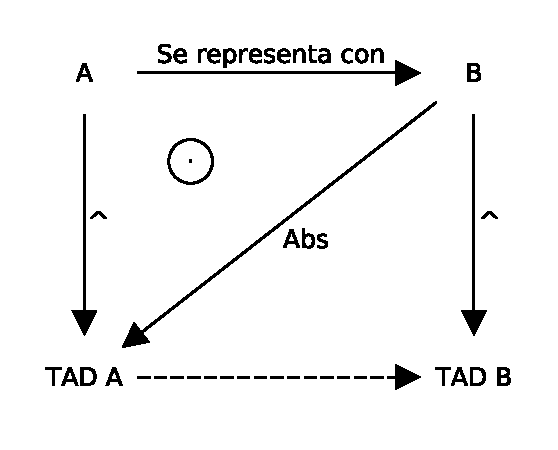
\includegraphics[width=0.3\textwidth]{graficos/FuncionDeAbstraccion.pdf}
 \caption*{\footnotesize $A$ ser\'a el modulo en cuesti\'on que estaremos dise\~nando y $B$ la estructura de representaci\'on del mismo. El circulo con el punto dentro hace alusi\'on al hecho de que la conmutaci\'on del triangulo conserva la sanidad. Esto significa que la aplicaci\'on de la funci\'on de abstracci\'on a $B$ deber\'a dar el mismo resultado que la aplicaci\'on de $\widehat{\text{\textbullet}}$ a $A$.
 \newline 
 \newline }
\end{SCfigure}

Tendremos dos formas de describir la funci\'on de abstracci\'on. La primera de ellas, en funci\'on de sus observadores b\'asicos. Dado que los observadores identifican de manera un\'ivoca al objeto del cual hablan, si nosotros describimos el valor que tienen los observadores b\'asicos una vez aplicados al objeto, estaremos describiendo desde un punto observacional pero sin ambig\"uedad el objeto representado. Otra forma de describir la funci\'on de abstracci\'on es utilizando los generadores del tipo de representaci\'on. La elecci\'on de elegir una forma u otra de hacerlo depende de la comodidad y declaratividad.

Dicho de otra forma, el objetivo de la funci\'on de abstracci\'on es poner en consonancia el tipo de soporte del modulo abstracto con los observadores del tipo que esta siendo representado. Una de las formas de realizar esto es caracterizando el valor de todos los observadores del TAD en base a valores de la instancia de la estructura de representaci\'on, de esa forma obtiene una instancia del TAD en consonancia con el modulo abstracto.

\subsubsection{Algoritmos}

En este paso se implementar\'an las operaciones del tipo a dise\~nar en t\'erminos de operaciones de los tipos soporte. Deben aparecer los algoritmos de cada una de las operaciones, sean \'estas de la interfaz o auxiliares. En el caso de las funciones auxiliares, es recomendable incluir junto a sus algoritmos, sus precondiciones y postcondiciones. En el dise\~no de los algoritmos hay que tener en cuenta que las operaciones deben satisfaces sus pre/postcondiciones, y adem\'as deben satisfacer los requerimientos de eficiencia surgidos en el contexto de uso.

\subsubsection{Servicios usados}

Aqu\'i es donde indicaremos qu\'e responsabilidades le dejamos a los tipos soporte que usamos. Son las pautas y requerimientos que se extraen del dise\~no de este tipo para el dise\~no de los tipos de la representaci\'on. Luego pasar\'an a ser las interfaces y los contextos de uso y requerimientos de eficiencia para los m\'odulos de soporte de los tipos usados en la representaci\'on.
